\chapter{Appendix}

\section{Detailed Transparency Report and DNS Abuse Mitigation by Cloudflare}
\label{app:cloudfare}


\begin{itemize}
    \item \textbf{Abuse Reports and Actions Taken}
    \begin{enumerate}
        \item Handling Abuse Reports: Clouderfare deals with various types of DNS abuses, including phishing, malware, and copyright infringement issues.
        \item Termination of Services: 
        \begin{itemize}
            \item Suspended Accounts and Dom: By the last half of 2022, Cloudflare suspended 206 accounts and 530 domains on proven grounds of association with hosting content for Child Sexual Abuse Material (CSAM).
        \end{itemize}
        \item  Uniform Domain Name Dispute Resolution Policy (UDRP) Requests: It managed 21 UDRP requests by dispute resolution boards approved by ICANN in the latter half of 2022, reflecting how serious Cloudflare is for the amicable resolution of domain disputes.
        \end{enumerate}
    \item \textbf{Law Enforcement and Legal Compliance}
    \begin{enumerate}
        \item Legal Sufficiency Review: Each request will be reviewed for legal sufficiency. Cloudflare will respond only to requests of this kind that meet the legal requirement, which refers to court orders and subpoenas.
        \item International Privacy Laws: Any requests that would contravene the right to privacy as subscribed to by laws of the involved countries are rejected, while bringing to the fore the subscription by Cloudflare to international legal standards.
        \item Emergency Disclosure Requests: Disclosures are made in situations that pose imminent harm, with a clear requirement for subsequent legal follow-up.
        \item National Security Requests: Cloudflare questions national security orders that are inconsistent with being a transparent organisation in the way it carries out its activities.
        \item International Data Requests: Review and respond to foreign government requests for compliance with US legal standard cases or case evaluations while maintaining the global perspective on privacy and legal integrity. 
    \end{enumerate}
    \item \textbf{Mitigation of DNS Abuse}
    \begin{enumerate}
        \item Public Reporting and Transparency:Cloudflare details and publicly reports these signals of abuse, both type and volume, so that there is transparency in the relationship of trust that makes the anti-abuse effort possible.
        \item Law Enforcement Cooperation: Continue your partnerships with law enforcement, ensuring that everything you do is justified from a legal perspective, particularly with regard to DNS abuse.
        \item Challenges to Mitigating DNS Abuse: It is also difficult to balance the obligation of the parties to legal rights with the need for collaborative and multi-stakeholder efforts to ensure DNS responsibility.
        \item Efficiency of efforts: Despite these challenges, Cloudflare mitigates abuse by working to address root causes and market diversity.
    \end{enumerate}
    \item \textbf{Proposals for Future Enhancements}
    \item Stakeholder Cooperation: Advocates for better cooperation in law enforcement, service delivery, and international organisations.
    \item Advances in Abuse Detection: Plans to invest in advanced technologies and machine learning to improve abuse detection and response times
    \item Trasparency Reporting : Commitment to further increase the frequency and level of detail in transparency reports, describing more clearly the nature and mitigation of DNS abuse. 
    \item User Education and Awareness: The organisation develops and distributes educational materials to increase the level of the user's awareness of the risks related to cybersecurity and DNS abuse.
    \item Policy and Legal Reforms: Engages toward advocating for policy and law changes to the resolution of any arising likely conflict between the privacy laws and law enforcement demands. 
    \item Multi-stakeholder Feedback Mechanism: Proposed to the Executive Board for adoption and implementation, which outlines feedback mechanisms to include input from users, civil society, and other stakeholders, which shall form the organisational bedrock for improvement and policy formulation.
        
    
\end{itemize}





\section{Presentation Slides}

\begin{figure}[H]
  \centering
  \begin{subfigure}[b]{0.55\linewidth}
    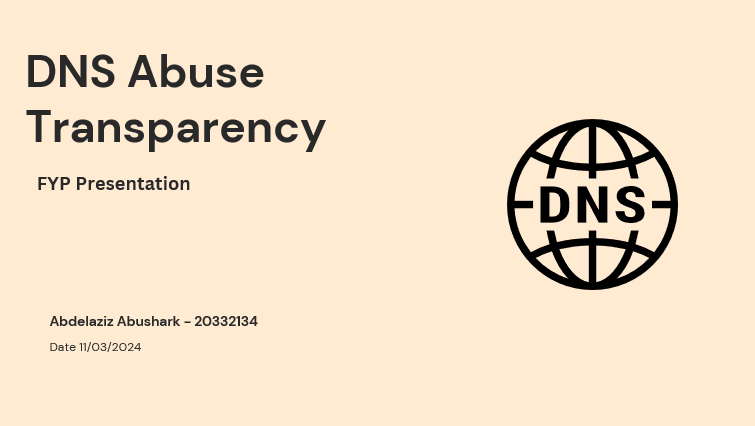
\includegraphics[width=\linewidth]{appendix/PRE1.png}
    \label{fig:left}
  \end{subfigure}
  \hfill % adds horizontal space between the figures
  \begin{subfigure}[b]{0.55\linewidth}
    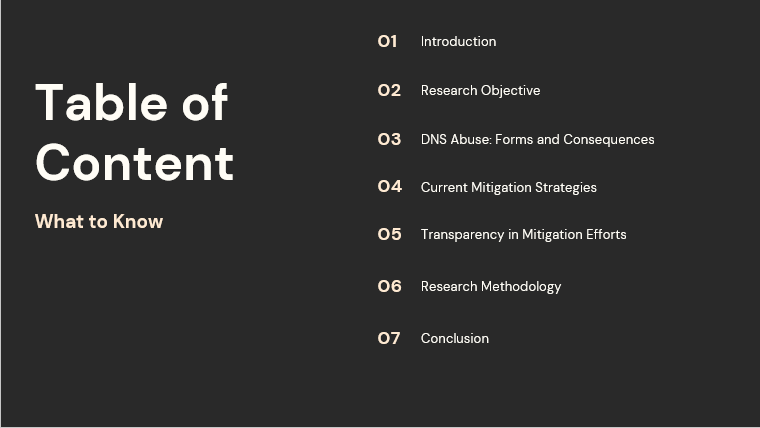
\includegraphics[width=\linewidth]{appendix/PRE2.png}
    \label{fig:right}
  \end{subfigure}
  \label{fig:images}
\end{figure}

\begin{figure}[H]
  \centering
  \begin{subfigure}[b]{0.55\textwidth}
    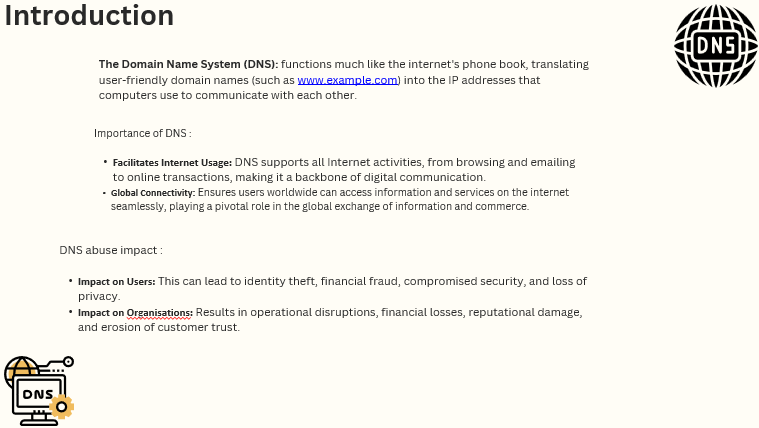
\includegraphics[width=\textwidth]{appendix/pre3.png}
    \label{fig:left}
  \end{subfigure}
  \hfill % adds horizontal space between the figures
  \begin{subfigure}[b]{0.55\textwidth}
    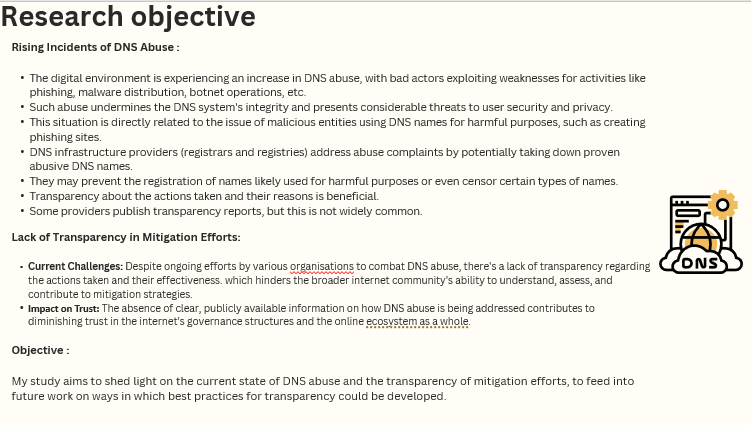
\includegraphics[width=\textwidth]{appendix/pre4.png}
    \label{fig:right}
  \end{subfigure}
  \label{fig:images}
\end{figure}

\begin{figure}[H]
  \centering
  \begin{subfigure}[b]{0.55\textwidth}
    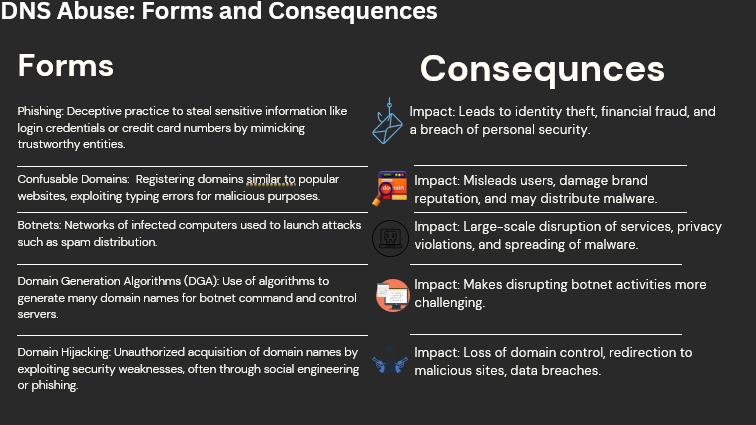
\includegraphics[width=\textwidth]{appendix/pre5.png}
    \label{fig:left}
  \end{subfigure}
  \hfill % adds horizontal space between the figures
  \begin{subfigure}[b]{0.55\textwidth}
    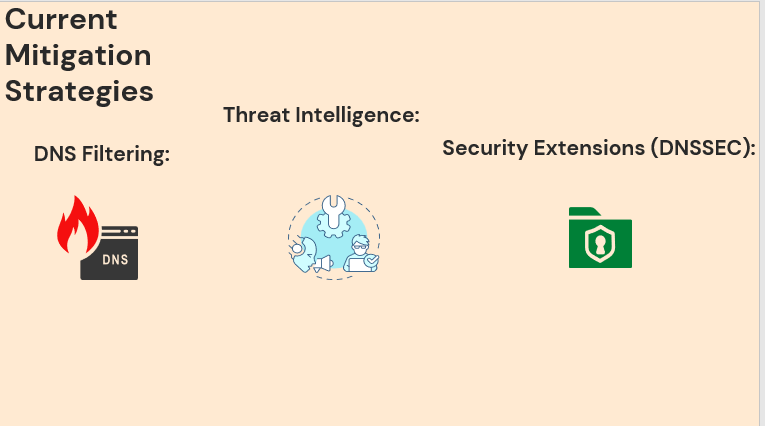
\includegraphics[width=\textwidth]{appendix/pre6.png}
    \label{fig:right}
  \end{subfigure}
  \label{fig:images}
\end{figure}

\begin{figure}[H]
  \centering
  \begin{subfigure}[b]{0.55\textwidth}
    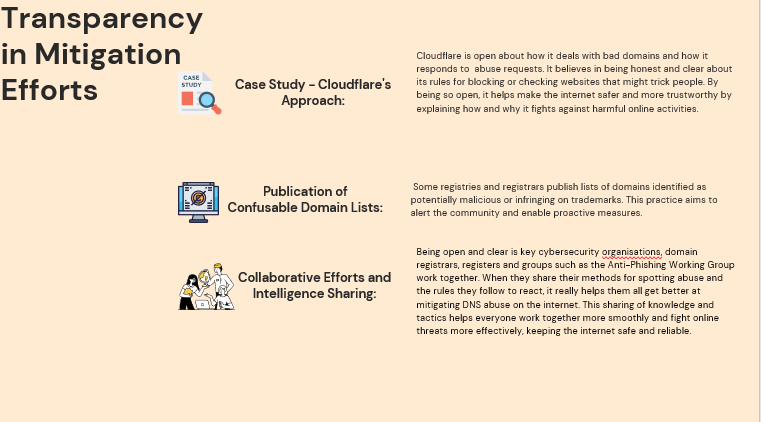
\includegraphics[width=\textwidth]{appendix/pre7.png}
    \label{fig:left}
  \end{subfigure}
  \hfill % adds horizontal space between the figures
  \begin{subfigure}[b]{0.55\textwidth}
    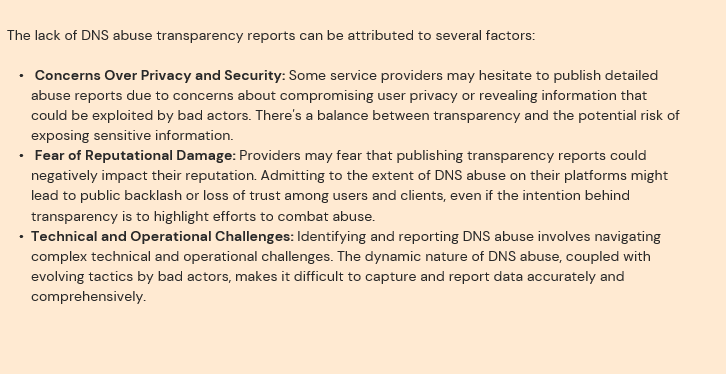
\includegraphics[width=\textwidth]{appendix/pre8.png}
    \label{fig:right}
  \end{subfigure}
  \label{fig:images}
\end{figure}

\begin{figure}[H]
  \centering
  \begin{subfigure}[b]{0.55\textwidth}
    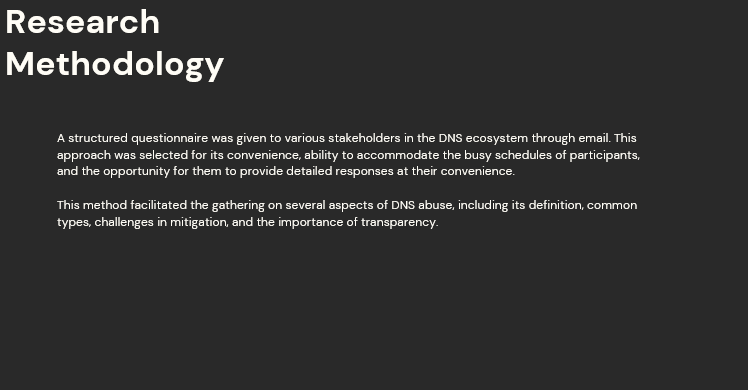
\includegraphics[width=\textwidth]{appendix/pre9.png}
    \label{fig:left}
  \end{subfigure}
  \hfill % adds horizontal space between the figures
  \begin{subfigure}[b]{0.55\textwidth}
    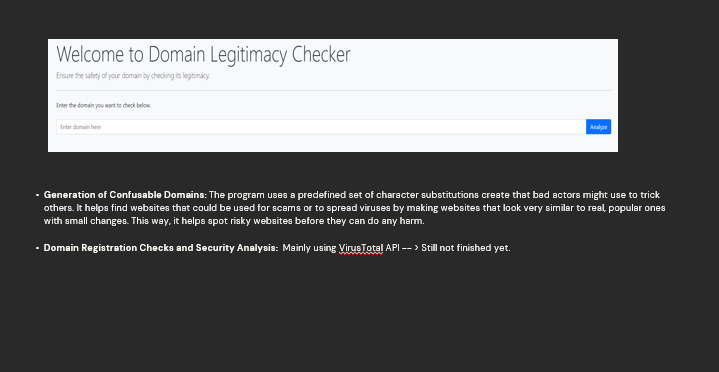
\includegraphics[width=\textwidth]{appendix/pre10.png}
    \label{fig:right}
  \end{subfigure}
  \label{fig:images}
\end{figure}

\begin{figure}[h]
    \centering
    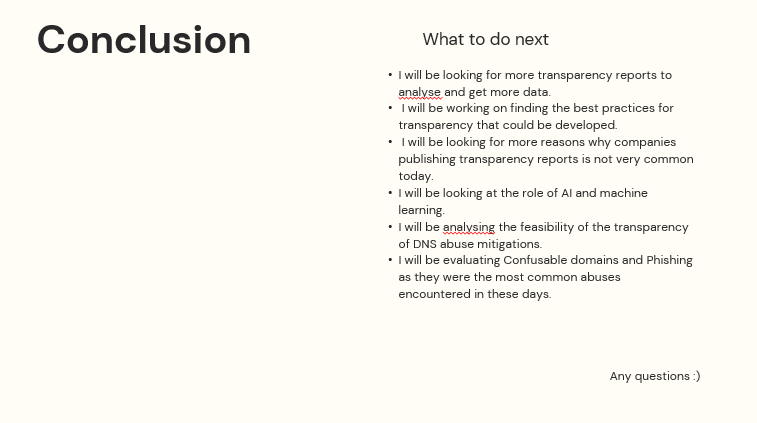
\includegraphics[width=0.55\linewidth]{appendix/pre11.png}
    \label{fig:lol}
\end{figure}